\documentclass{beamer}
\usetheme{CambridgeUS}
\usepackage[utf8]{inputenc} 
\usepackage{amsmath}
\usepackage[T1]{fontenc}
\usepackage{graphicx}
\usepackage{algpseudocode}
\usepackage{algorithm}
\usepackage{biblatex}
\usepackage{float}
\usepackage{tikz}
\usepackage[french]{babel}


\begin{document}

\title{CYK Probabiliste}  %PAGE 1
\author{ Arthur Lapraye \& Korantin Lévêque \& Mélanie Viegas }

\institute{Paris VII}
\date{\today}

\addtobeamertemplate{footline}{\insertframenumber/\inserttotalframenumber}

\begin{frame}
 \maketitle
\end{frame}

\begin{frame}
 \frametitle{Les PCFG}
 \begin{itemize}
  \item<1-4>{Les CFG : un quadruplet $(\Sigma,V,S,P)$ }
  \item<2-4>{Les CFG pondérées : ajout d'une fonction $ f : p \mapsto \alpha, p \in P, \alpha \in \mathbb{R} $ }
  \item<3-4>{Les CFG probabilistes : toutes les réécritures d'un non-terminal doivent sommer à 1. \\ $\forall X \in V \sum_{X\to\alpha\in R}p(X\to\alpha)=1$ }
  \item<4>{Les CFG probabilistes représentent un modèle de prédiction déduit à partir du corpus dont elles sont extraites.}
 \end{itemize}

\end{frame}

\begin{frame}
\frametitle{L'Algorithme CYK}
\begin{itemize}
  \item<1-4>{Un algorithme de parsing ascendant}
  \item<2-4>{Complexité $\mathcal{O}(|G|n^3) $ } %
  \item<3-4>{Parsing tabulaire}
  \item<4>{Extention aux grammaire hors-contexte probabilistes (PCFG)}
 \end{itemize}
 
\end{frame}

\begin{frame}
 \frametitle{L'Algorithme CYK}
%Ici on met le pseudo-code de l'algorithme

\end{frame}

\begin{frame}
 \frametitle{Transformer la grammaire en CNF}
 \begin{itemize}
  \item<1-4>
 \end{itemize}

 
\end{frame}



% \begin{frame} % PAGE 2
% \frametitle{Plan}
% \tableofcontents
% \end{frame}

\begin{frame}
  \frametitle{Le corpus Sequoia}
  \begin{columns}
  \begin{column}{0.5\textwidth}
    \begin{itemize}
     \item Un corpus diversifié
     
    \end{itemize}
   
  \end{column}
  
  \begin{column}{0.5\textwidth}
  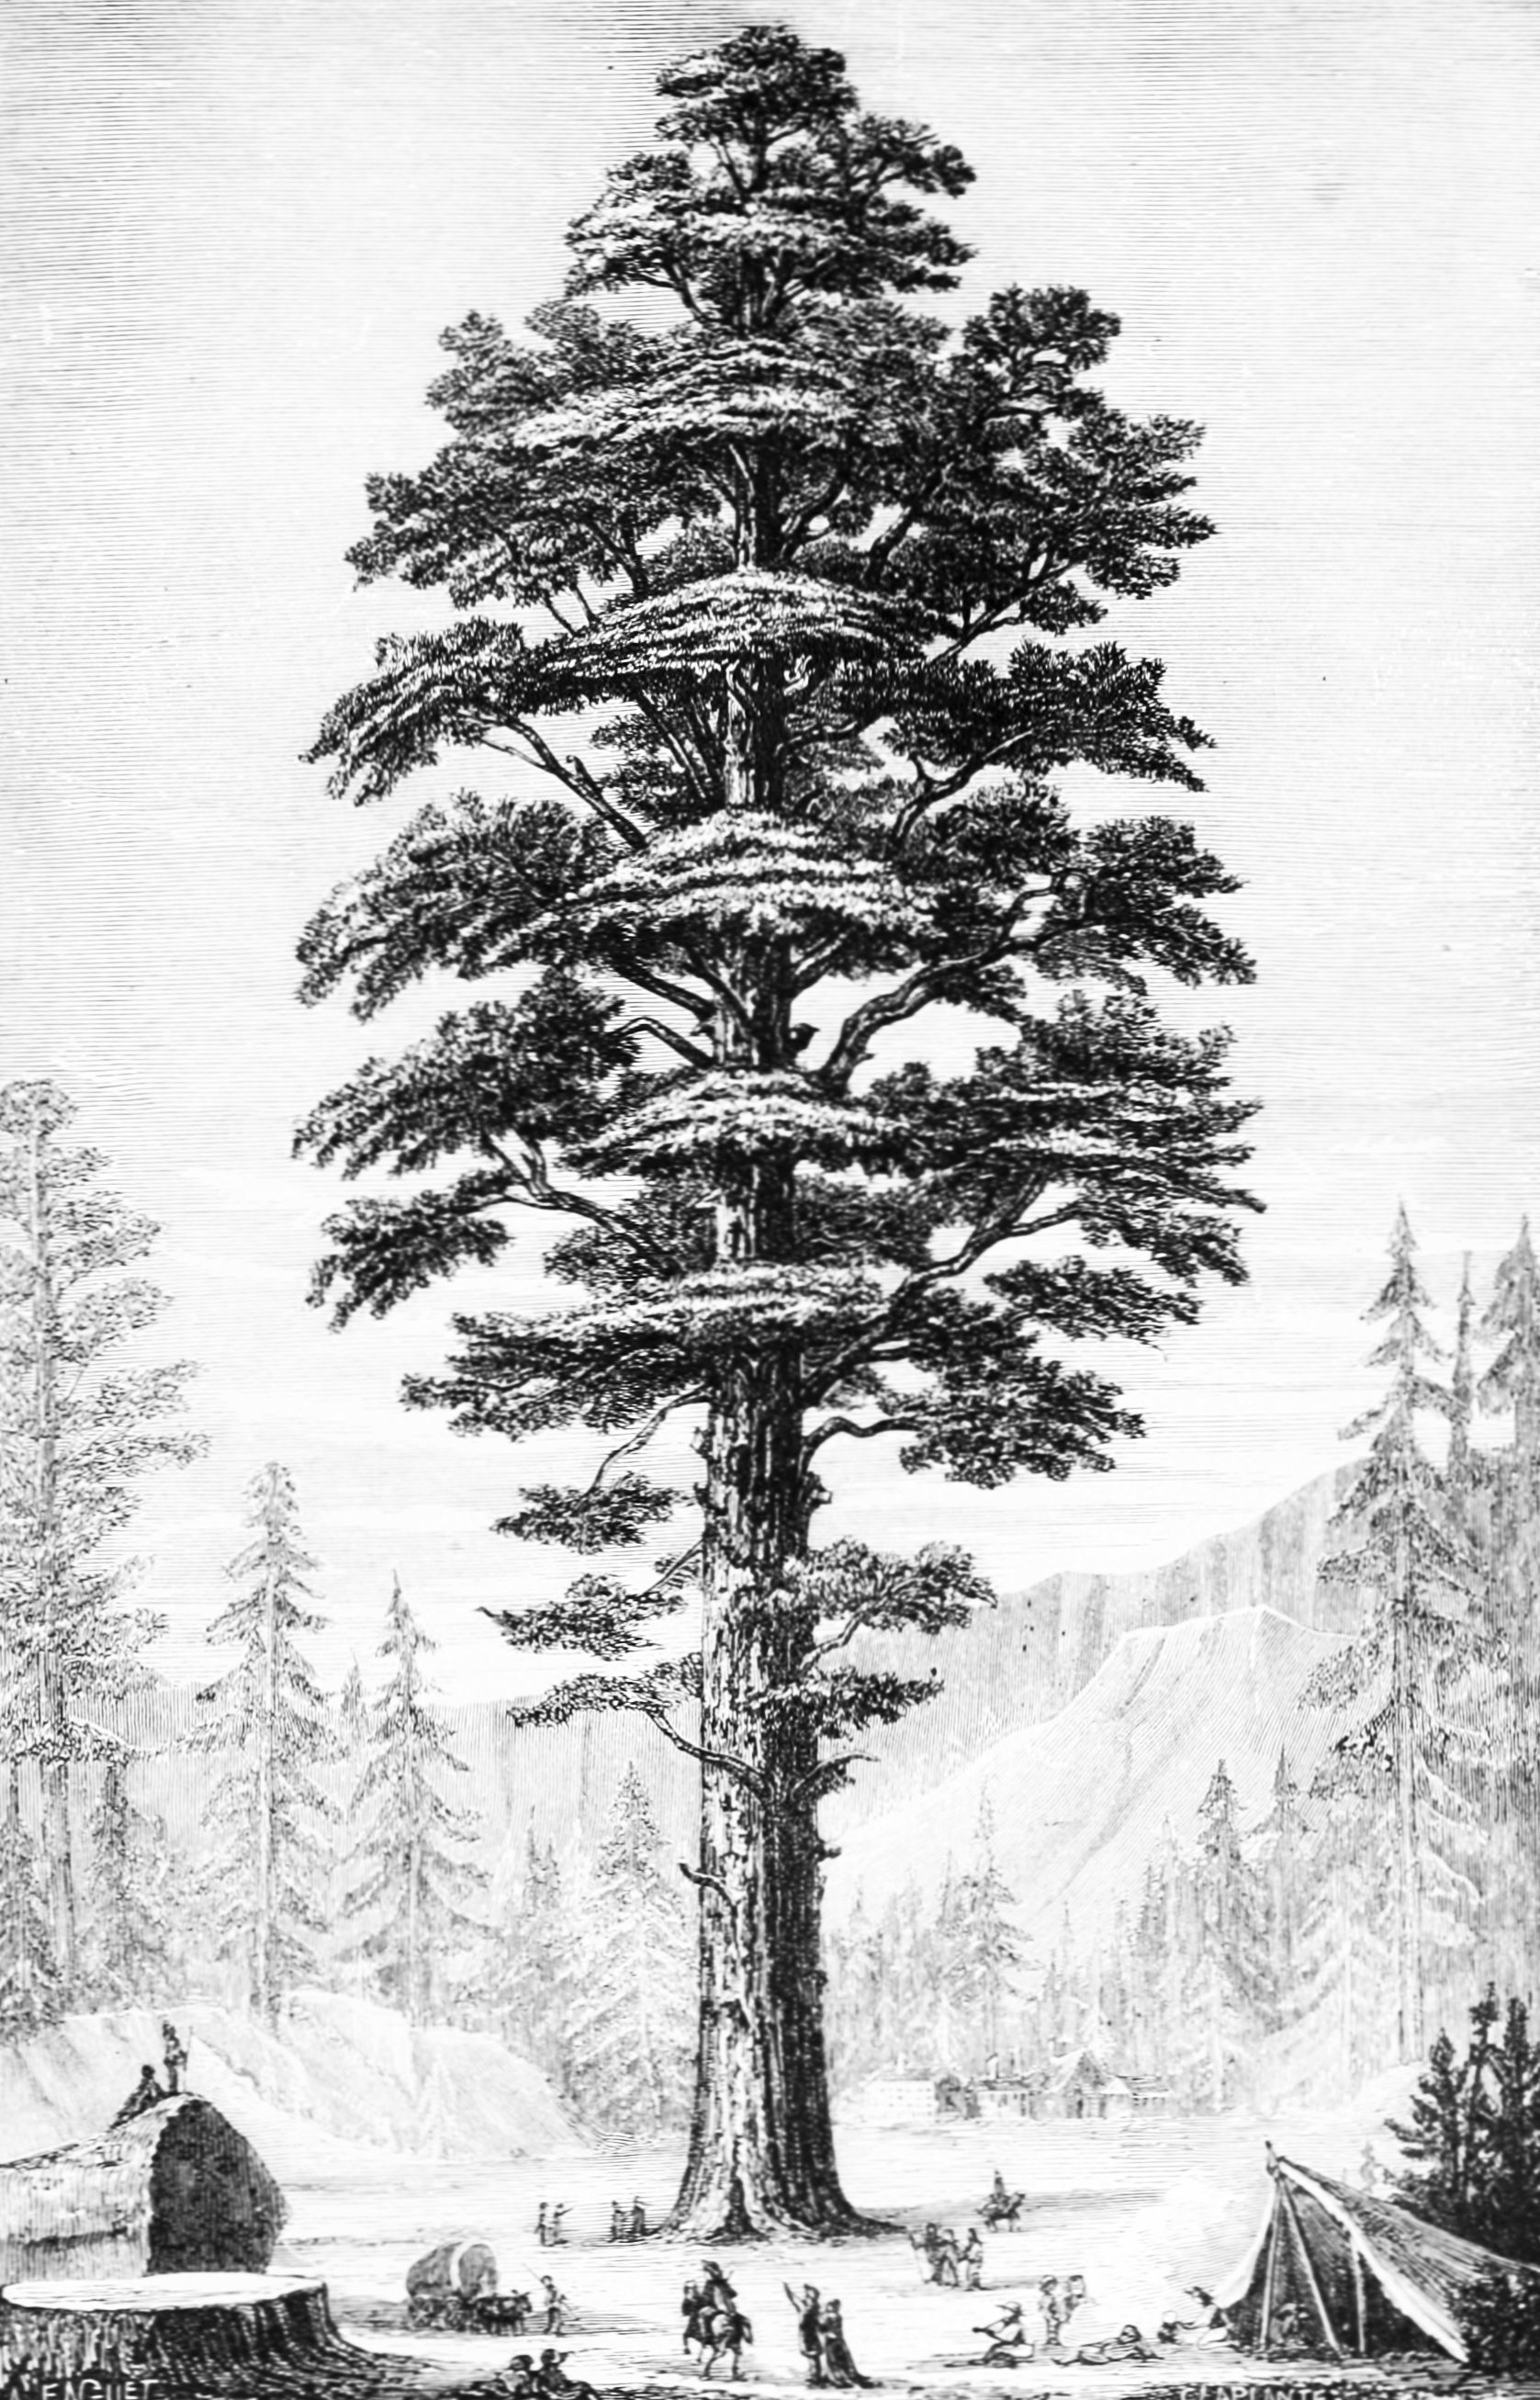
\includegraphics[width=80pt,]{PSM_V03_D341_Sequoia_gigantea_of_california.jpg}  
  \end{column}

  \end{columns}

\end{frame}

\begin{frame}
\frametitle{Notre implémentation du CYK}

 
\end{frame}

\begin{frame}
\frametitle{Evaluation}

\end{frame}



\begin{frame}{References}
  \begin{thebibliography}{5}    
  \beamertemplatebookbibitems
  \bibitem{roark}
    Brian Roark, Richard Sproat.
    \newblock {\em Computational Approaches to Morphology and Syntax}.
    \newblock Oxford University Press, 2007.
  \beamertemplatearticlebibitems
  \bibitem{parserEval}
    Mariana Romanyshyn, Vsevolod Dyomkin.
    \newblock {\em The Dirty Little Secret of Constituency Parser Evaluation}, 2014.
    \newblock {http://tech.grammarly.com/blog/posts/The-Dirty-Little-Secret-of-Constituency-Parser-Evaluation.html}
   \bibitem{LangeLeiss}
    Martin Lange, Hans Leiss
    \newblock{« To CNF or not to CNF : An Efficient Yet Presentable Version of the CYK Algorithm », 2009}
    \newblock{{\em Informatica Didactica} \No 8}
    
    \bibitem{BlackAbney}
     E. Black, S.Abney et al. 
    \newblock{« Procedure for Quantitatively Comparing the Syntactic Coverage of English Grammars »}
    \newblock{1991, DARPA Speech and Natural Language Workshop}
  
  \end{thebibliography}
\end{frame}


\end{document}
